\documentclass[11pt]{beamer}
\usefonttheme[onlymath]{serif}
\usepackage[utf8]{inputenc}
\usepackage{appendixnumberbeamer}
\usepackage{listings}
\usepackage{color}
\usepackage{textcomp}
\usepackage{lmodern}
\usepackage{ragged2e}
\usetheme{Frankfurt}
\usepackage{graphicx}
\usepackage{tikz}
\usetikzlibrary{shapes,arrows}
\usepackage{amsmath}
\author{Tom Hubrecht}
\graphicspath{{./Images/}}

%% Beamer Options %%
\setbeamertemplate{navigation symbols}{}

\setbeamertemplate{footline}
{
	\leavevmode%
	\hbox{%
		\begin{beamercolorbox}[wd=.4\paperwidth,ht=2.25ex,dp=1ex,center]{author in head/foot}%
			\usebeamerfont{author in head/foot}\insertshortauthor
		\end{beamercolorbox}%
		\begin{beamercolorbox}[wd=.6\paperwidth,ht=2.25ex,dp=1ex,center]{title in head/foot}%
			\usebeamerfont{title in head/foot}\insertshorttitle\hspace*{3em}
			\insertframenumber{} / \inserttotalframenumber\hspace*{1ex}
		\end{beamercolorbox}}%
	\vskip0pt%
}

\setbeamertemplate{section page}
{
	\begin{beamercolorbox}[sep=12pt,center]{part title}
		\usebeamerfont{section title}\insertsection\par
	\end{beamercolorbox}
}

\setbeamertemplate{subsection page}
{
	\begin{beamercolorbox}[sep=10pt,left]{part title}
		\usebeamerfont{subsection title}\insertsubsection\par
	\end{beamercolorbox}
}


\AtBeginSection{\frame[plain, noframenumbering]{\sectionpage}}
\AtBeginSubsection{\frame[plain, noframenumbering]{\subsectionpage}}


%% Create a font to use in the listings %%
%\newfontfamily\listingsfont[Scale=0.85]{droidsansmono.ttf}


%% Define colors for the listings %%
\definecolor{cred}{RGB}{255, 85, 85}
\definecolor{cgreen}{RGB}{85, 255, 85}
\definecolor{cblue}{RGB}{85, 85, 255}
\definecolor{cblack}{RGB}{0, 0, 0}
\definecolor{cwhite}{RGB}{255, 255, 255}


%% Listing Options %%
\lstdefinestyle{beamer}{
	backgroundcolor=\color{cwhite},   
	commentstyle=\color{cblack},
	keywordstyle=\color{cblue}\bfseries,
	numberstyle=\tiny\color{cblue},
	stringstyle=\color{cred},
	basicstyle=\ttfamily\scriptsize,
	breakatwhitespace=false,         
	breaklines=true,                 
	captionpos=b,                    
	keepspaces=true,                 
	numbers=left,                    
	numbersep=5pt,                  
	showspaces=false,                
	showstringspaces=false,
	showtabs=false,                  
	tabsize=3
}

\lstset{style=beamer}



\begin{document}
% Definition of blocks:
\tikzset{%
	block/.style    	= {draw, thick, rectangle, minimum height = 3em, minimum width = 3em},
	rsc/.style			= {draw, thick, rectangle, minimum height = 3em, minimum width = 4em},
	smallblock/.style 	= {draw, thick, rectangle, minimum height = 1em, minimum width = 1em, node distance = 2cm},
	sum/.style      	= {draw, circle, node distance = 1.5cm}, % Adder
	input/.style    	= {coordinate}, % Input
	output/.style   	= {coordinate} % Output
}

%Defining string as labels of certain blocks.
\newcommand{\suma}{\Large$+$}
\newcommand{\inte}{$\displaystyle \int$}
\newcommand{\derv}{\huge$\frac{d}{dt}$}
\newcommand{\inpt}{$\boldsymbol{\circ}$}

\title{Transmission d'informations entre la Terre et les sondes spatiales}
\date[]{269}

	
\begin{frame}[plain]
	\maketitle
\end{frame}

\begin{frame}[plain]{Table des mati\`eres}
	\tableofcontents
\end{frame}


\section{Introduction}
\subsection{Probl\'ematique}


\begin{frame}{Exploration spatiale}
	\centering
	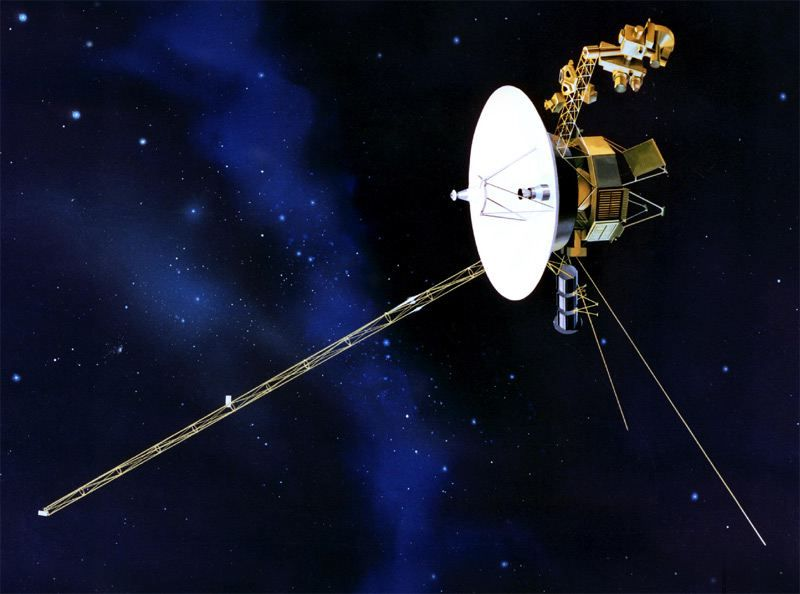
\includegraphics[scale=0.4]{VoyagerReverse}\\
	La sonde Voyager 2 communique avec le Terre alors qu'elle se trouve \`a 18 milliards de kilom\`etres.
\end{frame}


\subsection{Mod\'elisation}


\begin{frame}{Th\'eorie de l'information}
	\begin{tikzpicture}[auto, thick, node distance=2.5cm, >=triangle 45]
		\draw % Drawing the diagram of a communication system :
		node at (0, 0.9) {\small $Source$}
		node [block, name=source] {} 
		node at (2.5, 0.9) {\small $\acute{E}metteur$}
		node [block, right of=source] (emetteur) {}
		node at (4.5, 0.5) {\small $Canal$}
		node [smallblock, right of=emetteur] (canal) {}
		node at (6.5, 0.9) {\small $R\acute{e}cepteur$}
		node at (6.5, 0) [block] (recepteur) {}
		node at (9, 0.9) {\small $Destination$}
		node [block, right of=recepteur] (destination) {}
		node at (4.5, -3.1) [text width=2cm, text centered] {\small$Source$ $de$ $bruit$}
		node at (4.5, -2) [block] (bruit) {}
		;

		% Joining blocks. 
		% Commands \draw with options like [->] must be written individually
		\draw[->](source) -- node [below] {\scriptsize Message}(emetteur);
		\draw[->](emetteur) -- node [below] {\scriptsize Signal} (canal);
		\draw[->](canal) -- node [below] {\scriptsize Signal} (recepteur);
		\draw node at (5.3, -0.6) {\scriptsize re\c{ç}u};
		\draw[->](recepteur) -- node [below] {\scriptsize Message} (destination);
		\draw[->] (bruit) -- (canal);
	\end{tikzpicture}
\end{frame}

\begin{frame}{Cas de l'espace}
	\begin{itemize}	
		\item Canal de propagation gaussien
		\item Capacit\'e : $C = W.\log_{2}(1 + \frac{E_b}{N_0}) \; bit.s^{-1}$
		\begin{itemize}
			\item[-] $W$ : nombre de bits \'emis par seconde
			\item[-] $\frac{E_b}{N_0}$ : rapport signal sur bruit
		\end{itemize}
	\end{itemize}
\end{frame}


\section{Codes correcteurs d'erreurs}
\subsection{Principe}


\begin{frame}{Principe}
	\begin{itemize}
		\item Permettre de contrer l'action du bruit
		\item Se rapprocher de la limite de Shannon
	\end{itemize}
\end{frame}

\begin{frame}{D\'efinitions}
	\begin{itemize}
		\item Taux de transmission : $R = \frac{\text{nombre de bits du message}}{\text{nombre de bits envoy\'es}}$
		\item Probabilit\'e \`a posteriori (PAP)
		\item Rapport de vraisemblance logarithmique (LLR) : $\Lambda(d_k) = \log(\frac{\mathbf{P}(d_k = 1)}{\mathbf{P}(d_k = 0)})$
		%\item Codage syst\'ematique
	\end{itemize}
\end{frame}


\subsection{Diff\'erentes m\'ethodes}


\begin{frame}{Plusieurs classes de codes}
	\begin{itemize}
		\item Codes Reed-Solomon
		\item Codage par convolution
		\item Turbocodes
		\item Codes LDPC (Low Density Parity Checks)
	\end{itemize}
\end{frame}

\begin{frame}{Turbocodes}
	\centering
	
	\begin{tikzpicture}[auto, thick, >=triangle 45]
	\draw % Drawing the turbo encoder
	node at (0, 3) {\inpt}
	node at (0, 3.3) {\scriptsize $d_k$}
	node at (0.075, 3) [input] (stream) {}
	node at (2, 1.5) [input] (mid) {}
	node at (2, 0) [block] (interleaver) {\scriptsize Entrelaceur}
	node at (4, 1.5) [rsc] (rsc1) {Enc$_{1}$}
	node at (4, -1.5) [rsc] (rsc2) {Enc$_{2}$}
	node at (7, 3) [right] (xk) {$X_k$}
	node at (7, 1.5) [right] (y1k) {$Y_{1,k}$}
	node at (7, -1.5) [right] (y2k) {$Y_{2,k}$}
	;
	
	% Drawing the arrows
	\draw[->] (stream) -| (interleaver);
	\draw[->] (stream) -- (xk);
	\draw[->] (rsc1) -- (y1k);
	\draw[->] (rsc2) -- (y2k);
	\draw[->] (interleaver) |- (rsc2);
	\draw[->] (mid) -- (rsc1);
	\end{tikzpicture}
\end{frame}

\begin{frame}{Codes LDPC}
	\begin{itemize}
		\item Sommes de contrôles
		\item Multiplication matricielle
		\item Utilisation de matrices peu denses
	\end{itemize}
\end{frame}

\begin{frame}{Plusieurs types de d\'ecodage}
	\begin{itemize}
		\item D\'ecodage dur (Hard Decoding)
		\item D\'ecodage \`a d\'ecision douce (Soft decoding)
	\end{itemize}
\end{frame}


\section{Impl\'ementation des codes correcteurs}
\subsection{Choix des codes}


\begin{frame}{Codes utilis\'es}
	Les standards du CCSDS (Consultative Committee for Space Data Systems) pr\'econisent l'utilisation des Turbocodes et codes LDPC.
\end{frame}


\subsection{Repr\'esenter l'efficacit\'e des codes}


\begin{frame}{Choix de l'image}
	\begin{figure}
		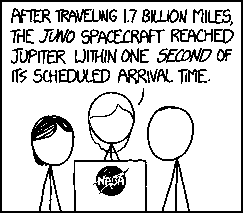
\includegraphics[scale=0.9]{base}
	\end{figure}
\end{frame}

\begin{frame}{Processus}
	\begin{itemize}
		\item Transformation de l'image en liste de bits
		\item Codage du message obtenu et transformation
		\begin{itemize}
			\item[] $0 \to -1.0$
			\item[] $1 \to 1.0$ 
		\end{itemize}
		\item Rajout d'un bruit blanc de moyenne nulle et de variance $s^2$
		\begin{itemize}
			\item[] $\frac{E_b}{N_0} = \frac{1}{s}$
		\end{itemize}
		\item Enregistrement du message bruit\'e
		\item D\'ecodage du message et enregistrement
		\item Recr\'eation des images obtenues \`a l'aide des listes de bits
	\end{itemize}
\end{frame}


\section{R\'esultats}
\subsection{Bruit faible}


\begin{frame}{Turbocodes, $\frac{E_b}{N_0} = 1.5$ dB}
	\begin{columns}
		\begin{column}{.5\textwidth}
			\begin{figure}
				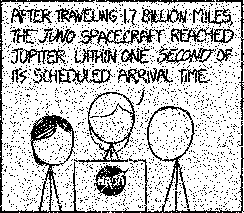
\includegraphics[scale=0.6]{turbo_noisy_70}\\
				Avant d\'ecodage
			\end{figure}
		\end{column}
		\begin{column}{.5\textwidth}
			\begin{figure}
				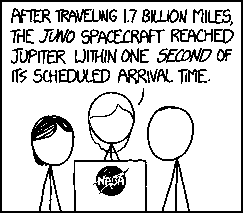
\includegraphics[scale=0.6]{turbo_decoded_70}\\
				Apr\`es d\'ecodage
			\end{figure}
		\end{column}
	\end{columns}
\end{frame}

\begin{frame}{Codes LDPC, $\frac{E_b}{N_0} = 2.2$ dB}
	\begin{columns}
		\begin{column}{.5\textwidth}
			\begin{figure}
				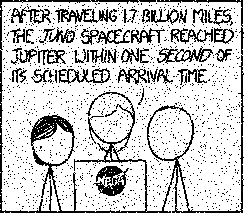
\includegraphics[scale=0.6]{ldpc_basic_noisy_60}\\
				Avant d\'ecodage
			\end{figure}
		\end{column}
		\begin{column}{.5\textwidth}
			\begin{figure}
				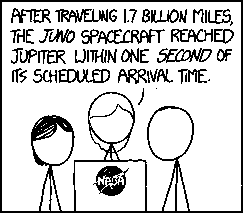
\includegraphics[scale=0.6]{ldpc_basic_decoded_60}\\
				Apr\`es d\'ecodage
			\end{figure}
		\end{column}
	\end{columns}
\end{frame}


\subsection{Bruit \'elev\'e}


\begin{frame}{Turbocodes, $\frac{E_b}{N_0} = 0.13$ dB}
	\begin{columns}
		\begin{column}{.5\textwidth}
			\begin{figure}
				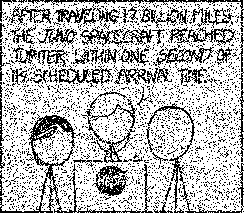
\includegraphics[scale=0.6]{turbo_noisy_97}\\
				Avant d\'ecodage
			\end{figure}
		\end{column}
		\begin{column}{.5\textwidth}
			\begin{figure}
				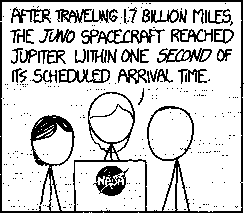
\includegraphics[scale=0.6]{turbo_decoded_97}\\
				Apr\`es d\'ecodage
			\end{figure}
		\end{column}
	\end{columns}
\end{frame}

\begin{frame}{Codes LDPC, $\frac{E_b}{N_0} = 0.97$ dB}
	\begin{columns}
		\begin{column}{.5\textwidth}
			\begin{figure}
				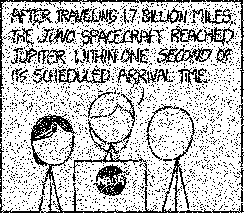
\includegraphics[scale=0.6]{ldpc_basic_noisy_80}\\
				Avant d\'ecodage
			\end{figure}
		\end{column}
		\begin{column}{.5\textwidth}
			\begin{figure}
				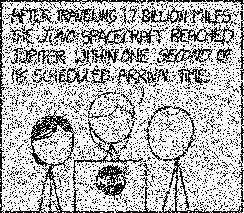
\includegraphics[scale=0.6]{ldpc_basic_decoded_80}\\
				Apr\`es d\'ecodage
			\end{figure}
		\end{column}
	\end{columns}
\end{frame}


\section*{Conclusion}



\appendix



\section{Code Informatique}

\begin{frame}[plain,fragile]{Transformation des images}
	\begin{lstlisting}[language=Python]
def image_to_bytes(file_name):
	cwd = os.getcwd()
	file_path = os.path.join(cwd, '..', 'files', 'images', file_name) + '.png'
	image = Image.open(file_path)
	
	data = list(image.getdata(band=0))  # The image is in grayscale
	
	byte_path = os.path.join(cwd, '..', 'files', 'bytes', file_name) + '.bt'
	try:
	byte_file = open(byte_path, 'xb')
	except FileExistsError:
	byte_file = open(byte_path, 'wb')
	
	for x in data:
	byte_file.write(x.to_bytes(1, 'big'))
	
	byte_file.close()
	\end{lstlisting}
\end{frame}

\begin{frame}[plain,fragile]
	\begin{lstlisting}[language=Python]
def bytes_to_image(file_name, size):
	cwd = os.getcwd()
	byte_path = os.path.join(cwd, '..', 'files', 'bytes', file_name) + '.bt'
	byte_file = open(byte_path, 'rb')
	
	image = Image.frombytes('L', size, byte_file.read(), "raw")
	file_path = os.path.join(cwd, '..', 'files', 'images', file_name) + '.png'
	try:
	file = open(file_path, 'xb')
	except FileExistsError:
	file = open(file_path, 'wb')
	
	image.save(file)
	file.close()
	image.close()	
	\end{lstlisting}
\end{frame}

\begin{frame}[plain, fragile]{Rajout de bruit}
	\begin{lstlisting}[language=C]
s_list * add_noise(h_list *mes, double s)
{
	s_list *res = csl(mes->n, mes->n);
	for (size_t i = 0; i < res->n; i++)
	{
		res->list[i] = (2 * mes->list[i]) - 1 + 
								box_muller(0, s);
	}
	return res;
}
	\end{lstlisting}
\end{frame}

\begin{frame}[plain, fragile]
	\begin{lstlisting}[language=C]
//(c) Copyright 1994, Everett F. Carter Jr.
double box_muller(double m, double s)
{
	double x1, x2, w, y1;
	static double y2;
	static int use_last = 0;
	if (use_last)
	{
		y1 = y2;
		use_last = 0;
	}
	else
	{
		do {
			x1 = 2.0 * (rand() / (double) RAND_MAX) - 1.0;
			x2 = 2.0 * (rand() / (double) RAND_MAX) - 1.0;
			w = x1 * x1 + x2 * x2;
		} while ( w >= 1.0 );
		
		w = sqrt( (-2.0 * log( w ) ) / w );
		y1 = x1 * w;
		y2 = x2 * w;
		use_last = 1;
	}
	
	return( m + y1 * s );
}
	\end{lstlisting}
\end{frame}

\begin{frame}[plain, fragile]{D\'ecodage basique}
	\begin{lstlisting}[language=C]
h_list * decode_h_basic(s_list *mes)
{
	h_list *res = chl(mes->n, mes->n);
	for (size_t i = 0; i < mes->n; i++)
	{
		res->list[i] = (mes->list[i] > 0);
	}
	return res;
}
	\end{lstlisting}
\end{frame}


\begin{frame}[plain, fragile]{Cr\'eation d'un code LDPC}
	\begin{lstlisting}[language=C]
h_matrix * create_base(size_t n, size_t j, size_t k)
{
    size_t m = (n * j) / k;
    h_matrix *res = chm(m, n);
    i_list *perm = cil(n, n);

    // Fill the first horizontal part of the matrix
    for (size_t i = 0; i < n; i++)
    {
        shm(res, 1, (i / k), i);
    }

    // Fill the j-1 other bands
    for (size_t i = 1; i < j; i++)
    {
        permutation(perm);
        for (size_t x = 0; x < n; x++)
        {
            shm(res, 1, ((perm->list[x] + i * n) / k), x);
        }
    }
    return res;
}
	\end{lstlisting}
\end{frame}

\section{Turbocodes}


\begin{frame}{Composant Enc}
	\centering

	\begin{tikzpicture}[auto, thick, node distance = 1.5cm, >=triangle 45, scale=0.95, every node/.style={transform shape}]
		\draw % Drawing the RSC component
		node at (-0.5, 3) {\inpt}
		node at (-0.5, 3.3) {\scriptsize $d_k$}
		node at (-0.425, 3) [input] (stream) {\inpt}
		node at (0, 3) [input] (mid) {}
		node [sum, right of=stream] (s1) {$+$}
		node [smallblock, right of=s1] (m1) {D}
		node [smallblock, right of=m1] (m2) {D}
		node [smallblock, right of=m2] (m3) {D}
		node [smallblock, right of=m3] (m4) {D}
		node [sum, below of=m1] (s2) {$+$}
		node [sum, below of=m3] (s3) {$+$}
		node [sum, below of=m4] (s4) {$+$}
		node [sum, above of=m3] (s5) {$+$}
		node [right of=s4] (out) {$Y_k$}
		;
		
		% Drawing the arrows
		\draw[->] (stream) -- (s1);
		\draw[->] (s1) -- (m1);
		\draw[->] (s1) -- (m1);
		\draw[->] (m1) -- (m2);
		\draw[->] (m2) -- (m3);
		\draw[->] (m3) -- (m4);
		\draw[->] (m4) |- (s5);
		\draw[->] (mid) |- (s2);
		\draw[->] (m1) -- (s2);
		\draw[->] (s2) -- (s3);
		\draw[->] (m3) -- (s3);
		\draw[->] (s3) -- (s4);
		\draw[->] (m4) -- (s4);
		\draw[->] (s5) -| (s1);
		\draw[->] (s4) -- (out);
	\end{tikzpicture}
\end{frame}

\subsection{D\'ecodage}
\begin{frame}{Sch\'ema d'un d\'ecodeur}
	Sch\'ema
\end{frame}

\begin{frame}{Processus de d\'ecodage}
	Le d\'ecodeur re\c{c}oit en entr\'ee trois variables r\'eelles pour le code avec $R = \frac{1}{3}$ :
	\begin{align*} \label{dec_input}
		x_k & = (2.X_k - 1) + a_k \\
		y_{1,k} & = (2.Y_{1,k} - 1) + b_k \\
		y_{2,k} & = (2.Y_{2,k} - 1) + c_k
	\end{align*}
	o\`u $a_k, b_k$ et $c_k$ sont des variables al\'eatoires suivant une loi normale de moyenne nulle et de variance $\sigma^2$
\end{frame}

\begin{frame}{Principe de d\'ecodage}
	On note $S_k$ l'\'etat de l'encodeur au moment k, $S_k = (a_k, a_{k-1}, a_{k-2}, a_{k-3})$ \\
	$S_0 = S_N = 0$ \\ \smallskip

	La sortie du canal fournie \`a l'entr\'ee du d\'ecodeur est la suite $R_1^N = (R_1,\ldots,R_k,\ldots,R_N)$
	o\`u $R_k = (x_k,y_{j,k})$ \\ \smallskip
	
	On introduit $\lambda_k^i(m) = \mathbf{P}(X_k = i, S_k = m / R_1^N)$, d'o\`u $\mathbf{P}(d_k = i / R_1^N) = \sum\limits_{m} \lambda_k^i$ et $\Lambda(X_k) = \log\left(\dfrac{\sum\limits_{m} \lambda_k^1}{\sum\limits_{m} \lambda_k^0}\right) $
\end{frame}

\begin{frame}
	On introduit des fonctions :
	\begin{itemize}
		\item $\alpha_k^i(m) = \dfrac{\mathbf{P}(X_k = i, S_k = m, R_1^k)}{\mathbf{P}(R_1^k)}.\mathbf{P}(X_k = i, S_k = m / R_1^k)$
		\item $\beta_k(m) = \dfrac{\mathbf{P}(R_{k+1}^N / S_k = m)}{\mathbf{P}(R_(k+1)^N / R_1^k)}$
		\item $\gamma_i(R_k, m', m) = \mathbf{P}(X_k = i, R_k, S_k = m/ S_{k-1} = m')$
	\end{itemize}
	On a par le calcul : $\lambda_k^i(m) = \alpha_k^i(m).\beta_k(m)$
\end{frame}

\begin{frame}{Algorithme de calcul}
	\begin{itemize}
		\item[-] \'Etape 0 : On initialise les probabilit\'es, \\
					$\qquad \alpha_0^i(0) = 1, \; \alpha_0^i(m) = 0 \quad \forall m \neq 0$\\
					$\qquad \beta_N(0) = 1, \; \beta_N(m) = 0 \quad \forall m \neq 0$
		\item[-] \'Etape 1 : Pour chaque inforation re\c{c}ue $R_k$, on calcule $\alpha_k^i(m)$, $\gamma_i(R_k, m', m)$
		\item[-] \'Etape 2 : Apr\`es la r\'eception du message, on calcule  $\beta_k(m)$ puis  $\lambda_k^i(m)$ et enfin $\Lambda(X_k)$
	\end{itemize}
\end{frame}


\section{Codes LDPC}
\subsection{Fonctionnement}


\begin{frame}{Principe math\'ematique}
	\begin{itemize}
		\item[-] Le codage comme multiplication matricielle dans $\mathbb{F}_2$
		\item[-] Utilisation de matrices peu denses $A \in \mathcal{M}_n(\mathbb{F}_2)$
		\item[-] Code (n, j, k)
	\end{itemize}
\end{frame}

\begin{frame}{G\'en\'eration d'un code LDPC}
	Utilisation de la m\'ethode de Robert Gallager pour un code (n, j, k).
	\begin{equation*}
	\begin{split}
	& A =
	\begin{pmatrix}
	A_1 \\
	A_2 \\
	\vdots \\
	A_j	\\ \end{pmatrix} \quad
	A_1 =
	\begin{pmatrix}
	1 & 1 & 1 & 0 & \cdots & 0 & 0 \\
	0 & 0 & 0 & 1 & \cdots & 0 & 0 \\
	\vdots & & & & \cdots & & \vdots \\ 
	0 & 0 & 0 & 0 & \cdots & 1 & 1 \\ \end{pmatrix}\\ & \\
	& \forall l \in {2, j}, \quad A_i = \left(C_{\sigma(1)}|\ldots|C_{\sigma(j)}\right) \text{o\`u} \; A_1 = \left(C_1|\ldots|C_j\right)
	\end{split}
	\end{equation*}

	La matrice de codage obtenue est alors $G = \begin{pmatrix} A \\ I \end{pmatrix}$ et la matrice de d\'ecodage $H = \begin{pmatrix} A & I \end{pmatrix}$
\end{frame}

\begin{frame}{Codage d'un message}
	Soit $m = (m_1, \ldots, m_n)$  un message \`a coder, on a $c = (c_1,\ldots,c_r)$ le message obtenu apr\`es codage,\\
	$c = G.m^T$  o\`u $r = \dfrac{nj}{k} + n$,

	Le taux de transmition vaut donc $R = \dfrac{k}{k + j}$

	Enfin, $H.c^T = 0$
\end{frame}


\subsection{D\'ecodage}


\begin{frame}{Repr\'esentation de Tanner}
	Un graphe de Tanner est associ\'e \`a la matrice de d\'ecodage H et comprend :
	\begin{itemize}
		\item $r$ noeuds messagers
		\item $\frac{n.j}{k}$ noeuds de contr\^ole
	\end{itemize}

	\centering

	\begin{tikzpicture}[auto, thick, node distance=1cm]
		\draw % Drawing the Tanner graph
		% Noeuds messagers
		node at (4.5, 4) {\textbf{Noeuds messagers}}
		node at (0, 3) [sum] (m1) {}
		node at (0, 3.4) {\scriptsize $m_1$}
		node [sum, right of=m1] (m2) {}
		node at (1.5, 3.4) {\scriptsize $m_2$}
		node [sum, right of=m2] (m3) {}
		node at (3, 3.4) {\scriptsize $m_3$}
		node at (4.5, 3) {$\cdots$}
		node at (6, 3) [sum] (m4) {}
		node at (6, 3.4) {\scriptsize $m_{r-1}$}
		node [sum, right of=m4] (m5) {}
		node at (7.5, 3.4) {\scriptsize $m_{r}$}
		% Noeuds de contrôle
		node at (4.5, 0) {\textbf{Noeuds de contr\^ole}}
		node at (0.75, 1) [smallblock] (c1) {}
		node at (0.75, 0.5) {\scriptsize $c_1$}
		node at (2.25, 1) [smallblock] (c2) {}
		node at (2.25, 0.5) {\scriptsize $c_2$}
		node at (4.5, 1) {$\cdots$}
		node at (6.75, 1) [smallblock] (c3) {}
		node at (6.75, 0.5) {\scriptsize $c_{\frac{nj}{k}}$}
		;
		
		% Drawing the links
		\draw[-] (c1.north) -- (m1);
		\draw[-] (c1.north) -- (m2);
		\draw[-] (c2.north) -- (m1);
		\draw[-] (c2.north) -- (m3);
		\draw[-] (m2) -- (3.7, 2.2);
		\draw[-] (c3.north) -- (m4);
		\draw[-] (c3.north) -- (m5);
		\draw[-] (c3.north) -- (5.3, 1.8);
	\end{tikzpicture}
\end{frame}

\begin{frame}{Plusieurs m\'ethodes}{D\'ecodage brut}
	\begin{itemize}
		\item Traduction du message re\c{c}u \`a l'aide d'une fonction seuil
		\item Calcul des sommes au niveau des noeuds de contr\^ole
		\item Modification des noueds messagers reli\'es aux noeuds de contrôles non satisfaits
		\item It\'eration jus'\`a satisfaction des noeuds de contr\^ole o\`u it\'eration maximale atteinte
	\end{itemize}
\end{frame}

\end{document}
